\chapter{Background and Methods} \label{chap:lit_rev}

As discussed in the previous chapter, such a complicated process as landslide simulation could be solved as a Fluid Structure Interaction (FSI) problem. It is well known in the CFD field, attacking researchers and scientists with different approaches. The main criteria and difficulty for the problem we consider in the current thesis are that we are solving a two-way coupling simulation \cite{benra2011comparison}. That means that simulations from the fluid part affect simulation from the solid part and vice versa, and we need to consider the best way to communicate between these two parts.

First, we describe formulation to solve fluid equations and free surface reconstruction, then the numerical method for its approximated solution. Then, consider the immersed boundary and discrete element method with the contact model.

We will start with Navier-Stokes system of equation for incompressible fluid which consist of momentum and continuity equation:

\begin{equation}\label{NS_methods}
\frac{\partial(\rho \mathbf{u})}{\partial t}+\nabla \cdot(\rho \mathbf{u u})=-\nabla p+\nabla \cdot \boldsymbol{\mu}+\rho \mathbf{g},
\end{equation}
\begin{equation}
\nabla \cdot \mathbf{u}=0,
\end{equation}
where $\mathbf{u}$ is the velocity vector field, $\rho$ is the fluid density, $p$ - the pressure, $\mu$ is the viscosity and $\mathbf{g}$ gravity force.

There is no analytical solution available for Navier Stokes equation; in fact, solution existence and uniqueness have not been proven till these days \cite{klay}. The most common and stable approach for fluid simulation is the finite volume method (FVM) \cite{ferziger2002cfd}, where we use the Eulerian frame of reference to solve momentum and continuum equations as a Navier-Stokes system.

\section{The finite volume method}
To solve \ref{NS_methods} we need to discretize the solution domain which is in turn give us a computational mesh on which governing equations are subsequently solved. The procedure is consist of two parts: discretisation of time and discretisation of space.

For the space discretisation we use Finite Volume Method (FVM), where the main feature is that domain is subdivided into Control Volumes (which is does not overlap and cover the whole domain).
\begin{equation}\label{2.2}
\frac{\partial\phi}{\partial t} +\nabla \cdot(\rho\mathbf{u}\phi) = \nabla \cdot(D \nabla \phi) + \nabla S ,
\end{equation}
where $D$ -  is diffusivity of the $\phi$ and $S$ is the source term. If we will write the equation in integral form as:
\begin{equation}
\int_{V_C} \frac{\partial\phi}{\partial t} d V+\int_{V_C} \nabla \cdot(\rho\mathbf{u}\phi) d V = \int_{V_C} \nabla \cdot(D \nabla \phi) d V + \int_{V_C} S d V,
\end{equation}
where $V_C$ is a fixed control volume $C$ and $S$ its flux over the boundaries. Then applying Gauss theorem to the convective and diffusive term we will get
\begin{equation}\label{2.3}
\frac{\partial}{\partial t}\int_{V_C} \phi d V+\int_{S_C} \nabla \cdot(\mathbf{u}\phi) d \mathbf{S} = \int_{S_C} \nabla \cdot(D \nabla \phi) d \mathbf{S} + \int_{V_C} S d V,
\end{equation}
where integral over a surface $S_C$ of control volume $C$ integral with normal directed outwards from control volume.
\subsection{Governing equations and domain discretization}
Using finite difference approach to propagate in time and replacing $\mathbf{u}$ by an approximation of the Taylor series around the cell centre.

Eqn. \ref{2.3} is semi-discretized form of eqn. \ref{2.2}, in order to solve it we need to approximate each term:

\begin{equation}
    \frac{\partial}{\partial t}\int_{V_C} \phi d V = \frac{ \rho^{n+1} \phi^{n+1} -  \rho^{n}\phi^{n} }{\Delta t} V_C
\end{equation}
for the forward Euler scheme:

\begin{equation}
    \int_{S_C}\nabla \cdot \rho\mathbf{u}_f \phi d \mathbf{S} \approx \sum_f  \rho\mathbf{u}_f \phi_f\cdot \mathbf{S}_f
\end{equation}
where $\mathbf{S}_f$ faces of the control volume element $C$ and $\mathbf{u}_{f}$ is interpolated value at the corresponding face.
Similar procedure applied for diffusive term if we assume that $D$ is a scalar
\begin{equation}
    \int_{S_C}\nabla\cdot(D \nabla \phi) d \mathbf{S} \approx \sum_f D (\nabla_f \phi)\cdot{d\mathbf{S}},
\end{equation}
where $ \nabla_f \phi$ is the face normal gradient at face $S_C$. The source term as a function of $\phi$ could be integrated over a the control volume as
\begin{equation}
\begin{array}{cc}
     &  S(\phi) = S_p\phi +S_u\\
     & \int_{V_C} S(\phi) d V  = S_p V_C\phi +S_u V_C
\end{array}
\end{equation}
where $S_p$ and $S_u$ are source terms.
%probably
%where $(\nabla p)_P$ is the pressure gradient at the centre of cell $P$. The pressure is calculated using Rhie-Chow\cite{rhie} interpolation scheme.


%\subsection{Equation discretization}
\subsection{Temporal discretization}
In order to propagate in time $[t, t+\Delta)$
\begin{equation}\label{2.5}
\int^{t+\Delta t}_t \left[\frac{\partial}{\partial t}\int_{V_C} \phi d V+\int_{S_C} \nabla \cdot(\rho \mathbf{u}\phi) d \mathbf{S}\right] d t=\int^{t+\Delta t}_t\left[\int_{S_C} \nabla \cdot(D \nabla \phi) d \mathbf{S} + \int_{V_C} S d V\right] d t
\end{equation}

Assuming that control volume does not change in time we can rewrite \ref{2.5} as a discretized form of transport equation \ref{2.2}. Using an implicit Euler formulation and substituting disrcetized spatial terms we will get:

\begin{equation} \label{NS_discr}
\frac{\rho^{n+1}\phi^{n+1}_C - \rho\phi^{n}_C}{\Delta t} V_{C}+\sum_{f} \mathbf{S}_{f} \cdot \rho\mathbf{u}_{f}\phi_f =\sum_{f} D_f\left(\mathbf{S}_{f} \nabla_{f} \phi_f^{n+1}\right)+ S_p V_C\phi^{n+1}_C +S_u V_C
\end{equation}
% c- is central flux probably???
where $\phi^{n+1}_C$ is the value of $\phi$ at the centre of control volume $C$ at time $t+\Delta t$, $\phi^{n}_C$ is the value of $\phi$ at the centre of control volume $C$ at time $t$, $\mathbf{S}_{f}$ is the area of face $f$, $\rho\mathbf{u}_{f}$ is the interpolated velocity at the face $f$, $\phi_f$ is the interpolated value of $\phi$ at the face $f$, $D_f$ is the diffusivity at the face $f$, $S_p$ and $S_u$ are source terms.

Face values have to be obtained from the neighboring cells, which is why interpolation scheme is play important role in accuracy and stability of the solution.

\subsection{Solving linear system of algebraic equations}
There are different approaches to get neighboring cell-face values. It could be widely used upwind scheme or it could be higher order scheme.

If we write \ref{NS_discr} in general form as:
\begin{equation}
a_{c} \phi_{c}^{n+1}+\sum_{N} a_{N} \phi_{N}^{n+1}=b_{c}
\end{equation}
where $N$ denotes of neighboring cells of $c$,  $a_c$ are the diagonal components of the matrix $[A]$ and $a_N$ are the off-diagonal components. This system could be written in a matrix form as:
\begin{equation}
[A][\phi]=\mathbf{B}
\end{equation}
where $[A]$ is the matrix containing the coefficients $a_c$ and $a_N$, $[\phi]$ is a flux values and $\mathbf{B}$ contains the source terms..

\subsection{Solution of the system}\label{p-v-coupling}
Because the momentum and continuity equation does not have a pressure relation \ref{NS_methods}, there are a couple of common ways to treat this issue \cite{ferziger2002cfd}. The most common are SIMPLE, PISO, and PIMPLE algorithms. This work uses Pressure Implicit Splitting Operator (PISO) \cite{ferziger2002cfd} due to its stability to time advantage. Equation
\begin{equation}\label{NS_algebraic}
    a_{P}^{\mathrm{u}} \mathbf{u}_{P}+\sum_{N} a_{N}^{\mathrm{u}} \mathbf{u}_{N}= -\nabla p,
\end{equation}
can be solved as a system of linear algebraic equations in two steps on a staggered according to the PISO approach. Usually, the pressure is calculated using the Rhie-Chow\cite{rhie} interpolation scheme. It is done to avoid pressure-velocity decoupling. The process of pressure-velocity coupling could be described in two steps:

\textbf{Step 1:} Prediction step, to find intermediate velocity:
\begin{equation}\label{NS_algebraic_1}
    (H+A)\mathrm{u} = -\nabla p^n
\end{equation}
where all non-diagonal elements stored in matrix $\mathbf{H}(\mathbf{u})= -\sum_{N} a_{N}^{\mathrm{u}} \mathbf{u}_{N}$ and diagonal elements stored in matrix $A$. Then we can rewrite \ref{NS_algebraic_1} as
\begin{equation}\label{NS_algebraic_2_}
    \begin{aligned}
a_{P}^{\mathrm{u}} \mathbf{u}_{P} &= \mathbf{H}(\mathbf{u})-\nabla p \\
\mathbf{u}_{P} &= \left(a_{P}^{\mathrm{u}}\right)^{-1}(\mathbf{H}(\mathbf{u})-\nabla p)
\end{aligned}
\end{equation}
where $P$ is an index arbitrary velocity node, $N$ is an index from neighbouring cells.

\textbf{Step 2:} Correction step, to find pressure and velocity:

Compute flux on a cell faces using Rhie-Chow \cite{rhie} correction
\begin{equation}
    \phi = \frac{H(\mathbf{u})}{a^u_P}\cdot S_f
\end{equation}
where $S_f$ is area of a cell face. From \ref{NS_algebraic_1} to satisfy continuity equation $\nabla\cdot \mathbf{u} = 0$
\begin{equation}
    (a_{P}^{\mathbf{u}})^{-1} \cdot \nabla^2 p^* = \nabla \cdot \phi,
\end{equation}
then correct the velocity field:
\begin{equation}
    \mathbf{u}^{*} = (a_{P}^{\mathbf{u}})^{-1}(H(\mathbf{u}) - \nabla p^*)
\end{equation}
where $\mathbf{u}^*$ and $p^*$, an intermediate velocity and a pressure. Then repeat step 2, until convergence condition is fulfilled and last step is writing down $\mathbf{u}^{n+1}$ and $p^{n+1}$ for the next step $n + 1$.

\section{Volume of fluid method for multiphase flow}

For multiphase flow simulation we are using as a base of Volume of Fluid Method (VOF) \cite{hirt1981vof}. The main idea of the method is to track the interface between two fluids by solving the continuity equation for the volume fraction of one of the fluids. The volume fraction is defined as the ratio of the volume of one fluid to the total volume of the two fluids.
\begin{equation}
\begin{array}{c}
\begin{aligned}
\frac{\partial(\rho \mathbf{u})_{i}}{\partial t}+\nabla \cdot(\rho \mathbf{u u})_{i} & = -\nabla p_{i}+\nabla \cdot \boldsymbol{\tau}_{i}+\rho_{i} \mathbf{g} \\
\nabla \cdot \mathbf{u}_{i} &= 0
\end{aligned}
\end{array}
\end{equation}
where $i$ is the phase number. The VOF method relays on finite volume mesh \cite{ferziger2002cfd}. For simulation of the free surface we add phase convection equation:
\begin{equation}
\frac{\partial \alpha}{\partial t}+\nabla \cdot(\alpha \boldsymbol{u})=0
\end{equation}
To differentiate fluid phases we can use scalar Heaviside step function to mark mesh cells as:
\begin{equation}\label{2.1}
\alpha(t, \mathbf{x})=\left\{\begin{array}{ll}
1, & \mathbf{x} \in \Omega_{1} \\
0, & \mathbf{x} \in \Omega_{2}, \cup \Gamma
\end{array}\right.
\end{equation}
where $\Omega_{1}$, $\Omega_{2}$ different fluid phases and $\Gamma$ is a surface. The surface $\Gamma$ is a free surface between two fluids.
\begin{figure}[!ht]
    \centering
    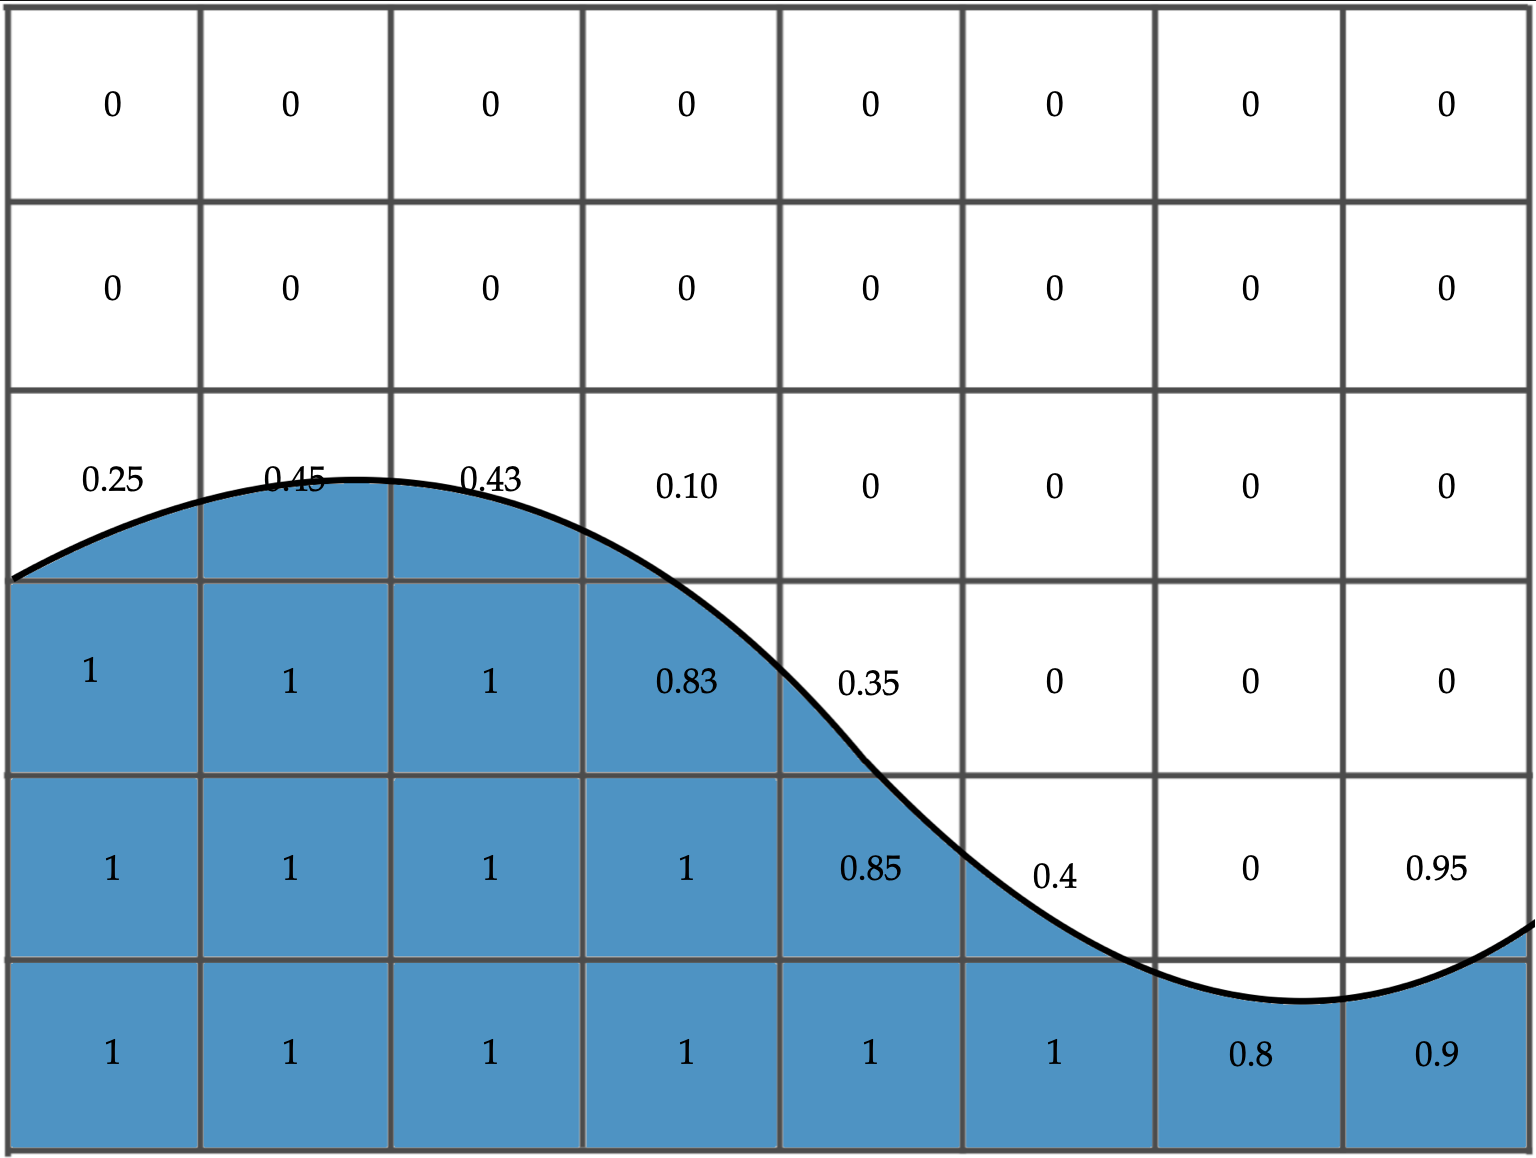
\includegraphics[width=9cm]{Images/VOF_free_surface.png}
    \caption{Schematic representation of volume of fluid mesh. Where values from $0$ to $1$ represent the fluid phase in a cell.}
    \label{fig:galaxy}
\end{figure}
On the interface boundary we need to satisfy equilibrium state:
\begin{equation}
\begin{array}{c}
\begin{aligned}
\left(\boldsymbol{\tau}_{1}-\boldsymbol{\tau}_{2}\right) \mathbf{e}&=\left(p_{1}-p_{2}+\sigma K\right) \mathbf{e} \\
\mathbf{u}_{1} &=\mathbf{u}_{2}
\end{aligned}
\end{array}
\end{equation}
where $\mathbf{e}$ - unit normal vector to $\Omega_1$, $K$ - surface curvature of $\Gamma$ and $\sigma$ is surface tension coefficient. Based on \ref{2.1} density and viscosity are:
\begin{equation}
\begin{array}{c}
\begin{aligned}
        \rho &= \alpha \rho_{\text {water}}+(1-\alpha) \rho_{\text {air}} \\
        \mu &= \alpha \mu_{\text {water}}+(1-\alpha) \mu_{\text {air}}
\end{aligned}
\end{array}
\end{equation}
In the pure advection problem with a predetermined velocity field the specific values of the fluid densities, $\rho_A$ and $\rho_B$ are immaterial, that is, the solution does not depend on them. To remove these insignificant parameters from the problem, we define the indicator field:
\begin{equation}
H(\mathbf{x}, t) \equiv \frac{\rho(\mathbf{x}, t)-\rho_{B}}{\rho_{A}-\rho_{B}}
\end{equation}
where $\rho_{A}$ and $\rho_{B}$ are the densities of the two fluids.

\section{Free surface reconstruction method}

The method discussed herein is a sharp interface reconstruction technique, often referred to by various authors as the geometric Volume of Fluid (VOF) approach. In their work, Deen et al. \cite{deen2009direct} utilized Direct Numerical Simulations (DNS) to simulate multi-phase flow, employing a combination of the VOF method \cite{hirt1981vof} and the Direct Forcing Immersed Boundary Method \cite{uhlmann2005immersed}. They used a piece-wise linear interface method for free surface reconstruction, as in the approach presented by Brackbill \cite{brackbill1992continuum}.

A noted limitation of the VOF method, as discussed in \cite{hirt1981vof}, arises when the mutual distance between bubbles is less than the size of a computational cell. This condition, referred to as mutual coalescence, makes mass conservation challenging. Consequently, alternate methods such as the Multidimensional Universal Limiter with Explicit Solution (MULES) \cite{zalesak1979fully} and isoAdvector \cite{roenby2019isoadvector} have been considered. The study by Roenby et al. \cite{roenby2019isoadvector} provides a comprehensive comparison of these two methods and proprietary solvers like ANSYS Fluent and STAR-CCM+, demonstrating their performance using a disk formation flow experiment. Roenby et al.'s work \cite{roenby2019isoadvector} gave promising results, with the source code available online. Because of performance and access to the source code, the free surface reconstruction approach from isoAdvector was tested and chosen.

The algorithm for isoAdvector,(\textbf{}) as described in detail by Roenby et al. \cite{roenby2019isoadvector}, consists of the following steps:
 
\begin{enumerate}
\item \textbf {Initialization:} The initial fluid distribution is represented by a field variable such as a color function or a volume fraction, which is set to $1$ in cells filled with fluid and $0$ in cells filled with air (or another fluid).
\item \textbf {Interface reconstruction:} The fluid-air interface is reconstructed in each cell based on the volume fraction. This is typically done using a geometric approach, which represents the interface as a planar surface within each cell
\item \textbf {Advection:} The interface is advected according to the local fluid velocity. This is done by sweeping a control volume through the cell in the friction of the velocity vector and computing the change in the volume fraction
\item \textbf {Correction:} After the advection step, the volume fractions are corrected to ensure mass conservation. This is done by adjusting the volume fraction in cells where the interface has been advected in or out.
\item \textbf {Update:} The new volume fractions are used to update fluid distribution for the next time step.
    %\item For each face calculate $\Delta V_j$ - total volume transported across cell $j$.
   % \item Choose all surface cells between $0 < \alpha < 1$.
   % \item Find isosurface inside the cell with Newton method. After it isosurface cuts the cell into 2 volumetric fractions.
   % \item Based on velocity field and velocity flux, estimate the isoface motion.
   % \item Calculate the face–interface intersection line.
  %  \item Use the motion of its face–interface intersection line to calculate $V_j$
  %  \item Based on $V_j$  calculate $\alpha$
  %  \item Adjust the $V_j$  for cell values $\alpha < 0$ or $\alpha > 1$
\end{enumerate}
%as schematically shown on the figure %\ref{}
%High Resolution Interface Capturing (HIRC) \cite{muzaferija1999two} STAR-CCM+ 
For isoAdvector method the amount of each phase calculated as:
\begin{equation}
    \alpha_{i}=\frac{1}{V_{i}} \int_{\Omega_{i}} H(\boldsymbol{x}, t) d V,
\end{equation}
where $V_i$ is the volume of cell $i$ and $\Omega_i$ surface??? represents each cell to calculate the phase fractions at the next time step. The volume fraction of each phase is then updated as: 
\begin{equation}\label{isoAd-2_}
    \alpha_{i}(t+\Delta t)=\alpha_{i}(t)-\frac{1}{V_{i}} \sum_{j \in B_{i}} s_{i j} \int_{t}^{t+\Delta t} \int_{F_{j}} H(\boldsymbol{x}, \tau) \boldsymbol{u}(\boldsymbol{x}, \tau) d \boldsymbol{S} d \tau
\end{equation}
Here, the flux of $\alpha$ across each cell face is time-integrated and then summed. The symbol $B_i$ denotes the set of all faces $F_j$ associated with cell $i$. The factor $s_{ij}$ is employed to direct the flux outward from the cell. $\tau$ is the integration variable used over the time step, and $dS$ is the differential area vector pointing out of the volume.

The factor $s_{ij}$ can either be $+1$ or $-1$. Its purpose is to ensure that the product $s_{ij}dS$ always points outward from the cell boundary, even when the orientation of face $j$ causes $dS$ to point into the cell.

The right side integrals could be replaced with $\Delta V_j(t,\Delta t)$, which represents the total volume of fluid transported across face $j$ during one time step in given by:
\begin{equation}\label{isoAd-1}
    \Delta V_{j}(t, \Delta t)=\int_{t}^{t+\Delta t} \int_{F_{j}} H(\boldsymbol{x}, \tau) \boldsymbol{u}(\boldsymbol{x}, \tau) d \boldsymbol{S} d \tau
\end{equation}
This allows us to experss the next step as: 
\begin{equation}
\alpha_{i}(t+\Delta t)=\alpha_{i}(t)-\frac{1}{V_{i}} \sum_{j \in B_{i}} s_{i j} \Delta V_{j}(t, \Delta t)
\end{equation}
In the context of fluid equations of motion treated by the finite volume method, the velocity field is naturally represented by cell-averaged values:
\begin{equation}
\mathbf{u}_{i}(t) \equiv \frac{1}{V_{i}} \int_{\mathcal{C}_{i}} \mathbf{u}(\mathbf{x}, t) d V
\end{equation}
Given that the convective terms in the governing fluid equations denote the transport of properties like mass and momentum across cell faces, another crucial step for representing the velocity field is the volumetric fluxes across mesh faces:
\begin{equation}\label{isoAd-3}
\phi_{j}(t) \equiv \int_{\mathcal{F}_{j}} \mathbf{u}(\mathbf{x}, t) \cdot d \mathbf{S}
\end{equation}
where $\phi_{j}$ is the face flux across the face $j$.
\subsection{The advection step}
Many interface flow solvers in the Navier-Stokes equations use a segregated solution approach, wherein the governing flow equations are solved sequentially for each time step. As a result, while advancing the interface from time $t$ to $t + \Delta t$, we only have access to the velocity field information up to time $t$. However, to compute the updated $\alpha i$ as illustrated in equation \ref{isoAd-2}, it's necessary to understand the velocity field within the interval [$t$, $t + \Delta t$]. This implies estimating how the velocity field evolves during this time step.

The most straightforward approach is to presume that the velocity field remains constant throughout the entire time step. This assumption simplifies the expression in equation \ref{isoAd-1} to $u(x, \tau) \approx u(x, t)$. Furthermore, in equation \ref{isoAd-1}, we suppose that the dot product of $u$ with the differential face normal vector, $dS$, on face $F_j$ can be approximated in terms of the volumetric face flux, $\phi_j$  \ref{isoAd-3} as:
\begin{equation}
\mathbf{u}(\mathbf{x}, t) \cdot d \mathbf{S} \approx \frac{\phi_{j}(t)}{\left|\mathbf{S}_{j}\right|} d S \text { for } \mathbf{x} \in \mathcal{F}_{j}
\end{equation}
if we set face normal as in \cite{roenby2019isoadvector}:
\begin{equation}
\mathbf{S}_{j} \equiv \int_{\mathcal{F}_{j}} d \mathbf{S}
\end{equation}
and substitute in into \ref{isoAd-1}, we will get:
\begin{equation}\label{isoAd-2}
\Delta V_{j}(t, \Delta t) \approx \frac{\phi_{j}(t)}{\left|\mathbf{S}_{j}\right|} \int_{t}^{t+\Delta t} \int_{\mathcal{F}_{j}} H(\mathbf{x}, \tau) d S d \tau
\end{equation}
while the the rest of the \ref{isoAd-2} is the area of the face $j$ submerged in one fluid, which we call $A_{j}(\tau)$:
\begin{equation}
A_{j}(\tau) \equiv \int_{\mathcal{F}_{j}} H(\mathbf{x}, \tau) d S=\int_{\mathcal{F}_{j} \cap \mathcal{A}(\tau)} d S
\end{equation}
Replace $A_{j}(\tau)$ into \ref{isoAd-2} we will get:
\begin{equation}
\Delta V_{j}(t, \Delta t) \approx \frac{\phi_{j}(t)}{\left|\mathbf{S}_{j}\right|} \int_{t}^{t+\Delta t} A_{j}(\tau) d \tau
\end{equation}
The transport of one fluid across a face is computed only once per face. For internal faces, this calculated value is utilized to update the volume fractions for both cells adjoining the face. This process ensures both local and global conservation of the two fluids, as discussed in \cite{roenby2019isoadvector}.
\section{Immersed boundary method}
First, the terminology was used in \cite{peskin1972flow} to study blood flow through the heart. The method has since been applied to various problems in fluid dynamics, solid mechanics, and biological systems. In the current method, solid bodies cover several computational cells. There are two primary approaches to handling fluid-structure interaction problems: body conformal mesh methods and fixed mesh methods. Body conformal mesh methods offer high accuracy but come with increased complexity in implementation and computational cost and are unsuitable for the simulation of granular media processes.

On the other hand, fixed mesh methods discretize the entire computational domain at once, with both fluid phases and solids sharing a single velocity and pressure field. This leads to more efficient calculations, making the fixed mesh approach the method of choice for this thesis. Figure \ref{fig:CFDDEM} provides a schematic representation of a solid body within a 2D fluid domain before and after discretization. 
\begin{figure}[!ht]
    \centering
    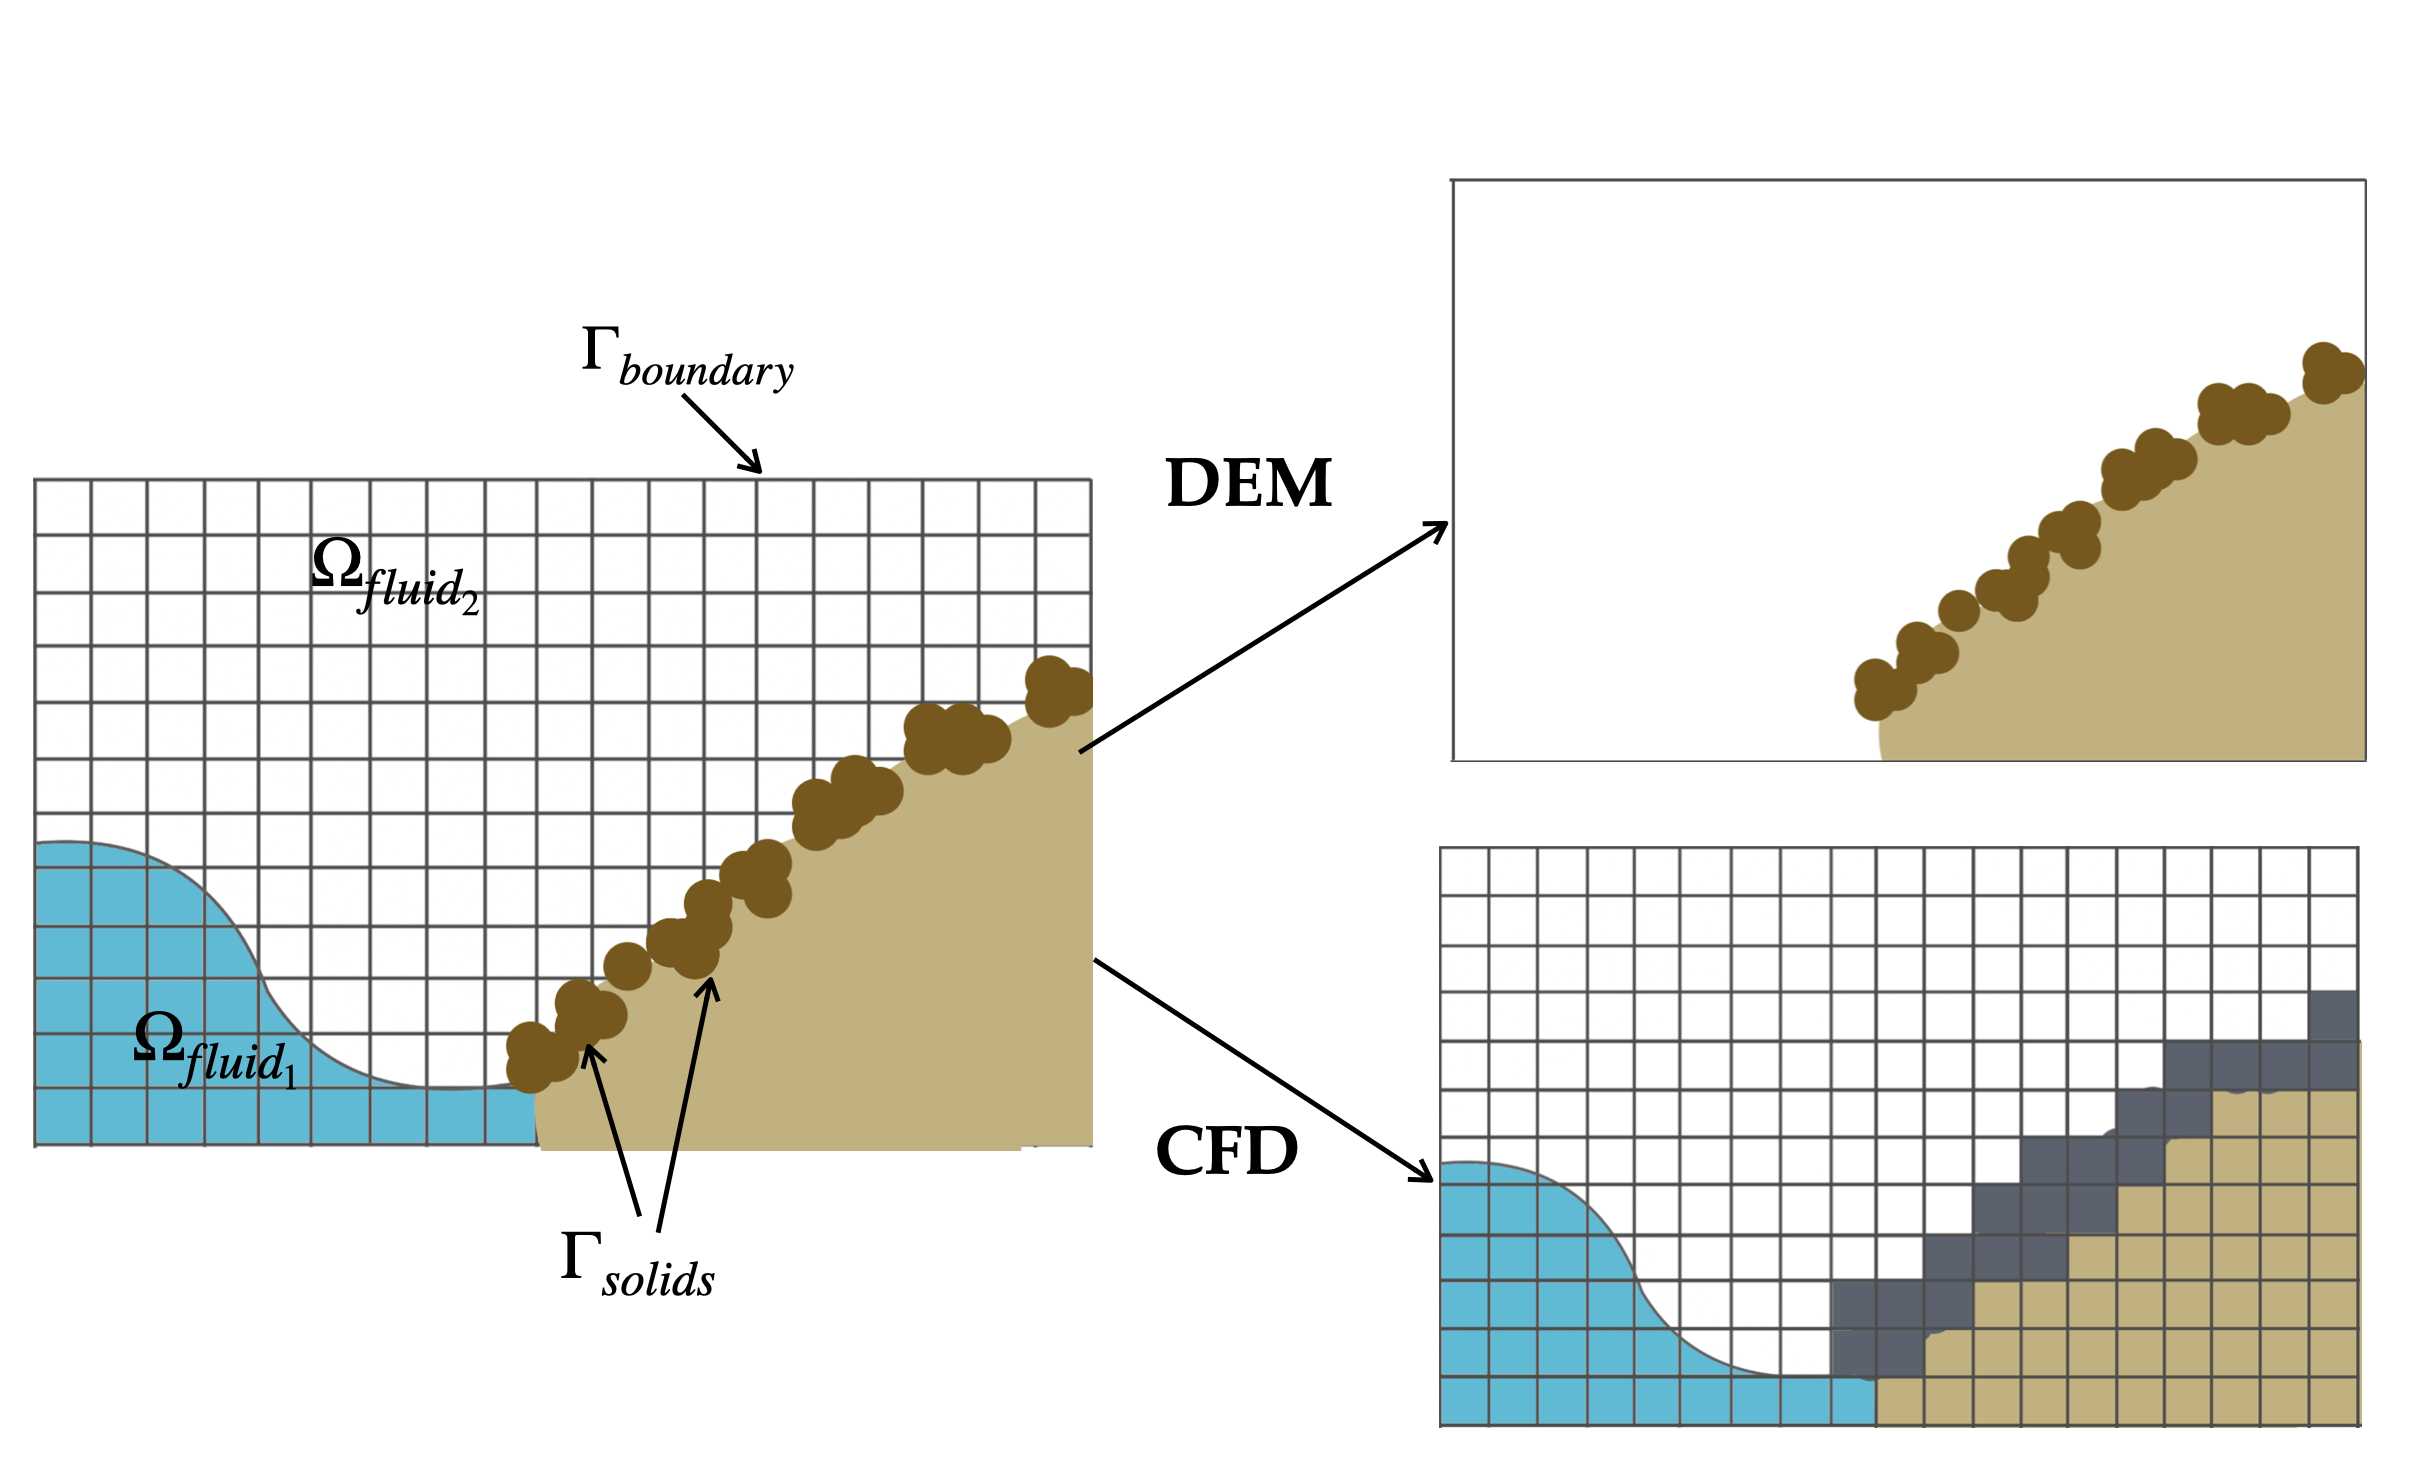
\includegraphics[width=14cm]{Images/CFD_DEM_scheme.png}
    \caption{Particle in the fluid domain (left), representation of the particle in DEM (top) and CFD (bottom).  $\Omega_{fluid_1}$ is the water domain, $\Omega_{fluid_2}$ the air phase, $\Omega = \Omega_{fluid}$. $\Gamma_{solid}$ is the interface between fluid and solid. 
}
    \label{fig:CFDDEM}
\end{figure}


\subsection{Void fraction calculation}

To account solid body on Eulerian mesh in CFDEMcoupling \cite{kloss2012models} used \textit{smooth representation} \cite{kloss2012models} algorithm where the each sphere of multisperical body divided into a core and corona and similar procedure done for each particle \ref{fig:core}. 

The \textit{voidFraction} $\beta_i$ model is used to calculate clump forces and correct the fluid velocity field. The main challenge is that particle dynamics are calculated in a Lagrangian coordinate system, while fluid dynamics use an Eulerian coordinate system. To account for the solid body on the Eulerian mesh, the CFDEMcoupling employs a \textit{smooth representation} algorithm \cite{kloss2012models}, where each sphere of a multispherical body is divided into a core and a corona as shown in Figure \ref{fig:core}. A similar procedure is done for each particle.
\begin{figure}[ht]
    \centering
    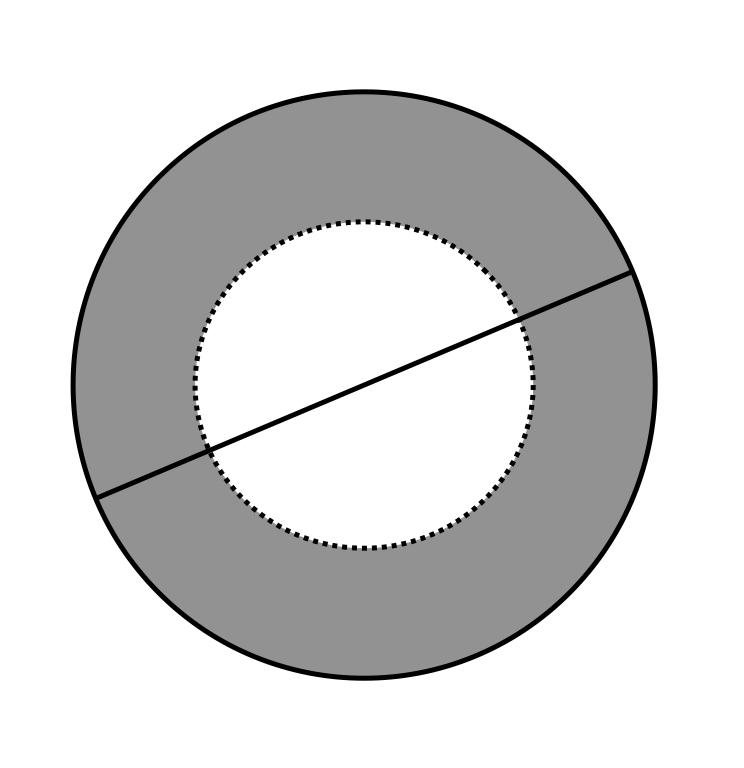
\includegraphics[width=6cm]{Images/chap3/core_corona.png}
    \caption{Schematic representation of the particle divided into core (white) and corona (gray).}
    \label{fig:core}
\end{figure}
All cells detected within the particle's area have their relative positions with respect to the particle checked. If they are located inside the core, their volume fraction is set to one. For cells covered by the corona, a loop over all vertices belonging to the cell begins. If the vertex is inside the particle, the cell's volume fraction is increased by one-eighth (since each cell has eight vertices in the given case). If the vertex lies outside the corona, the intersecting point of the particle hull and the connection between the cell center and edge is computed. The relative length of the line between the cell center and intersection, multiplied by one-eighth, is then added to the cell's current volume fraction. This method's verification has been made in the work by Kloss et al. \cite{kloss2012models}.

First we need to assign a weight for every finite volume cell 
\begin{equation}
\beta_{i}=\frac{N_{v c, i}+N_{c c, i} N_{v, i}}{2 N_{v, i}}
\end{equation}
where $N_{v c, i}$ and $N_{c c, i} $ are the number of vertices and centers intersecting the immersed body, respectively. $N_{v, i}$ one of the vertices, for haxahedral cell $i = 8$. The weight is used to calculate the velocity of the immersed body at the cell center. The velocity of the immersed body at cell $i$'s center is calculated as:
\begin{equation} \label{IB_forces}
    \boldsymbol{u}_{i b, i} = \boldsymbol{v}_{i b}+\frac{1}{N_{v c, \mathrm{i}}+N_{v, \mathrm{i}}}\left[\left(\sum_{j}^{N_{v, i}} \omega \times\left(\boldsymbol{x}_{v, j}-\boldsymbol{x}_{i b}\right)\right)+N_{v, i} \boldsymbol{\omega} \times\left(\boldsymbol{x}_{c, \mathrm{i}}-\boldsymbol{x}_{i b}\right)\right]
\end{equation}
The velocity of cell $i$, denoted as $\boldsymbol{u}_{ib, i}$, includes the translational velocity $\boldsymbol{v}_{ib}$ and the rotational velocity around the center of rotation $\boldsymbol{x}_{ib}$. The coordinates of the cell's center and vertices are represented by $\boldsymbol{x}_{c, \mathrm{i}}$ and $\boldsymbol{x}_{v, j}$, respectively. It is important to note that the angular component of the immersed body's velocity at cell $i$'s position cannot be determined analytically due to the stair-casing effect. The expression within the brackets represents this angular velocity, which is not precisely known.
However, for a fully covered cell, it is equivalent to the angular velocity at the cell center.
\begin{figure}[!ht]
    \centering
    \begin{minipage}[b]{0.47\textwidth}
        \centering
        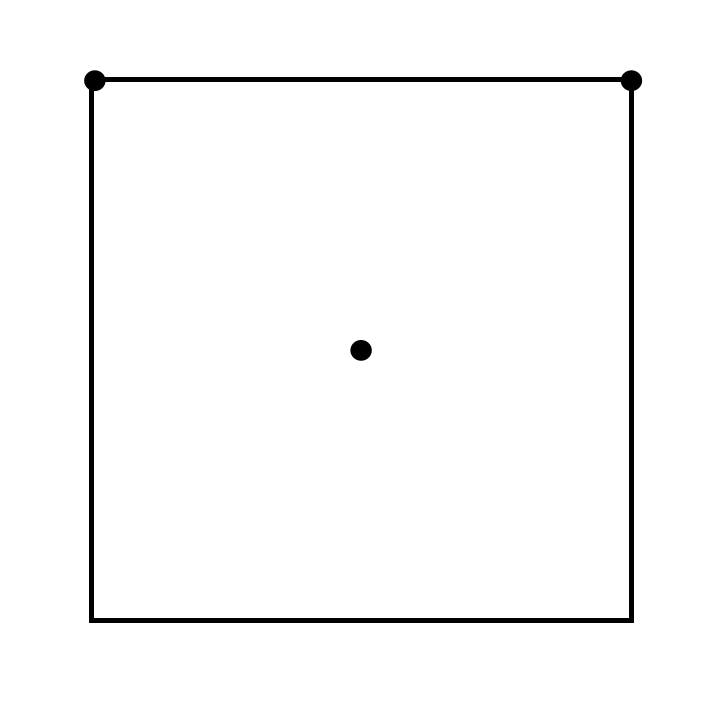
\includegraphics[width=5.8cm]{Images/chap3/1.png}
        \subcaption{}
    \end{minipage}
    \hfill
    \begin{minipage}[b]{0.47\textwidth}
        \centering
        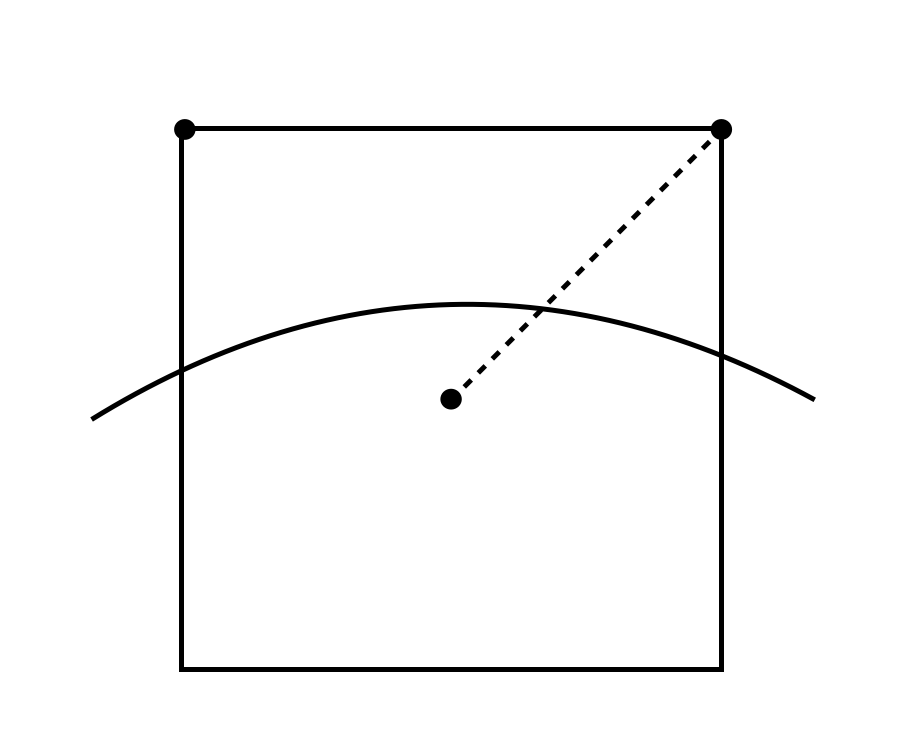
\includegraphics[width=\textwidth]{Images/chap3/2.png}
        \subcaption{}
    \end{minipage}
    
    \vspace{1em} % Add vertical space between rows

    \begin{minipage}[b]{0.47\textwidth}
        \centering
        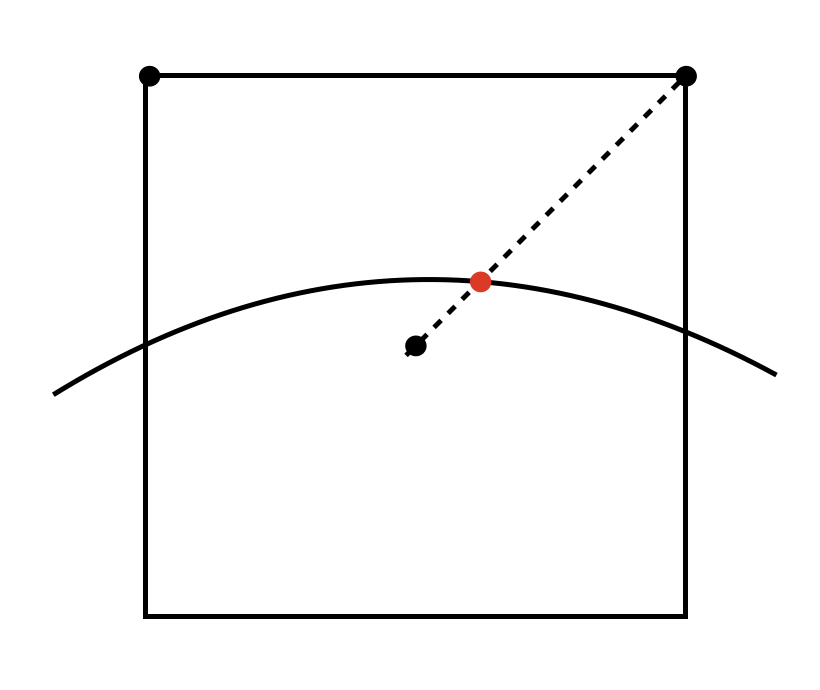
\includegraphics[width=\textwidth]{Images/chap3/3.png}
        \subcaption{}
    \end{minipage}
    \hfill
    \begin{minipage}[b]{0.47\textwidth}
        \centering
        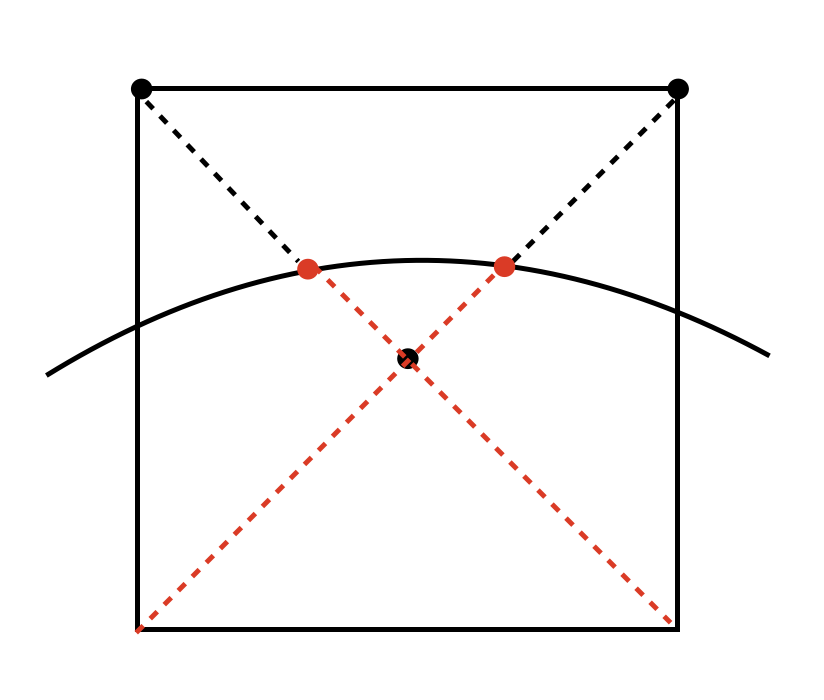
\includegraphics[width=\textwidth]{Images/chap3/4.png}
        \subcaption{}
    \end{minipage}

    \caption{Schematic representation of defining \textit{voidFraction} process: a)Vertex is outside the particle b) Connecting a line between the cell center and vertex c)Intersecting point of the particle hull and the connection between the cell center and edge is computed d)Summing up the contributions of all vertices}
    \label{fig:voidfraction-process}
\end{figure}

Using this methodology, the volume of the projected immersed body may not exactly match the volume enclosed by its surface mesh. Consequently, a halo layer is introduced to adjust the volume of the discretized immersed body. This layer corresponds to cells $i$ where the body fraction $\beta_i$ falls within the range of ]$0$, $1$[. Its size is modified to ensure the volume remains unaffected by cell alignment. The entire process is summarized in the block diagram depicted on the Figure \ref{fig:diag} below.
\begin{figure}[!htp]
    \centering
    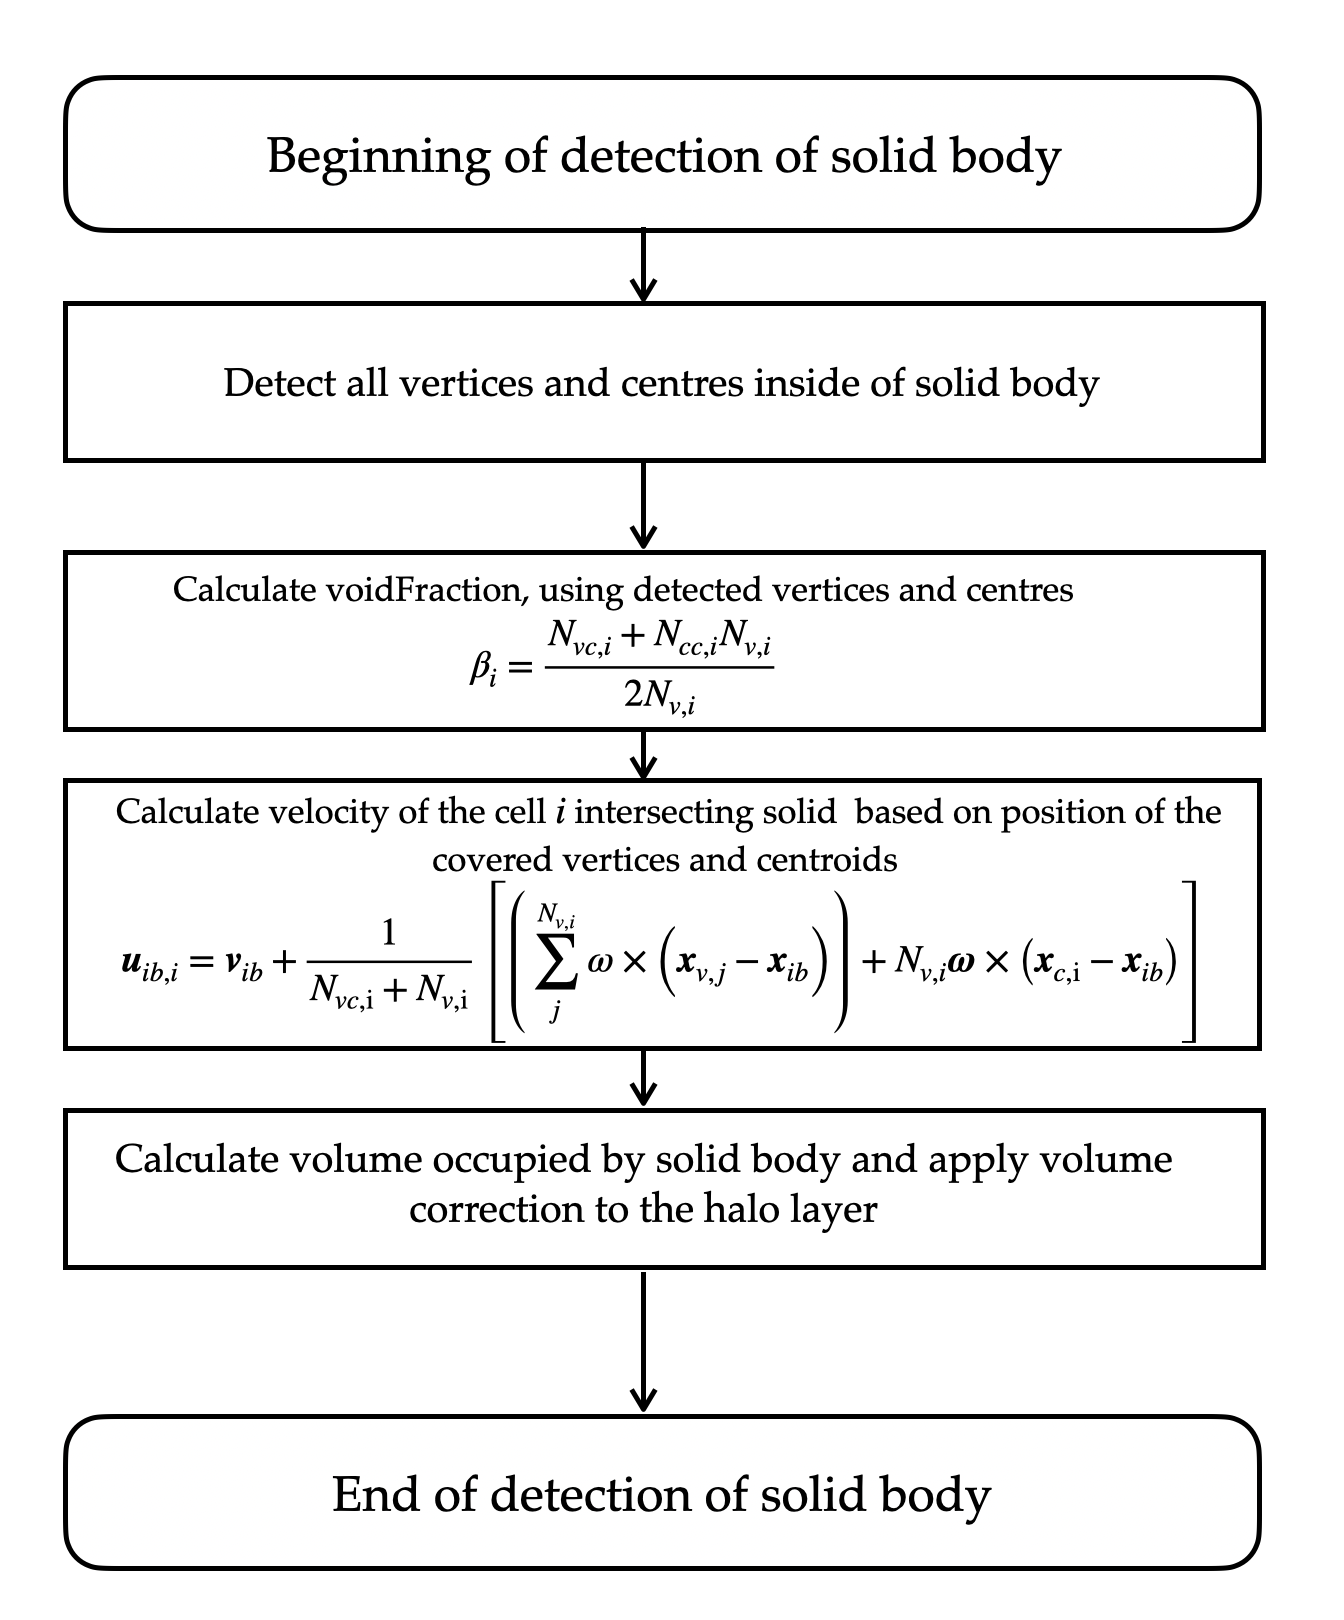
\includegraphics[width=12cm]{Images/chap3/diag.png}
    \caption{Schematic diagram for the defining process of the solid on the fluid mesh}
    \label{fig:diag}
\end{figure}
\section{Discrete element method}
The Discrete Element Method (DEM) serves as a foundational approach in the simulation of granular media and solid body motion. DEM models consist of two core components: the individual elements, particles like sand grains or stones, and the contacts between them. The first step in any DEM-based simulation is to establish a geometrical model, specify the mechanical properties of the elements and contacts, and define the time-varying loads on the system.

While perfectly spherical elements are computationally convenient, they often result in unrealistic behavior, particularly in non-cemented assemblies. This has been understood since the 1980s, leading to the use of 'clumps' for representing non-spherical particles. A clump is essentially a set of multiple overlapping spheres rigidly connected to approximate the shape of a complex particle. These clumps move as a single entity, effectively mimicking a particle with a more intricate shape. Graphical examples of clumps are shown in Figures \ref{fig:3figsA}, \ref{fig:3figsB}.

The use of clumps introduces some computational overhead due to the increased number of contact interactions and complexity in force calculations. However, this is still more efficient than directly simulating truly irregular shapes, which would require even more complex contact detection algorithms. The use of clumps is a straightforward and computationally efficient way to represent non-spherical particles in DEM simulations. By adjusting the number, size, and arrangement of spheres within a clump, various particle shapes can be approximated with varying levels of accuracy. Clumps can increase the computational cost of DEM simulations compared to simple spherical particles, as the number of contact interactions and the complexity of force calculations may increase. However, this approach is still more efficient than directly simulating irregular particle shapes, which would involve more complex contact detection and force calculations.
\begin{figure}[!htp]
\centering
\parbox{7cm}{
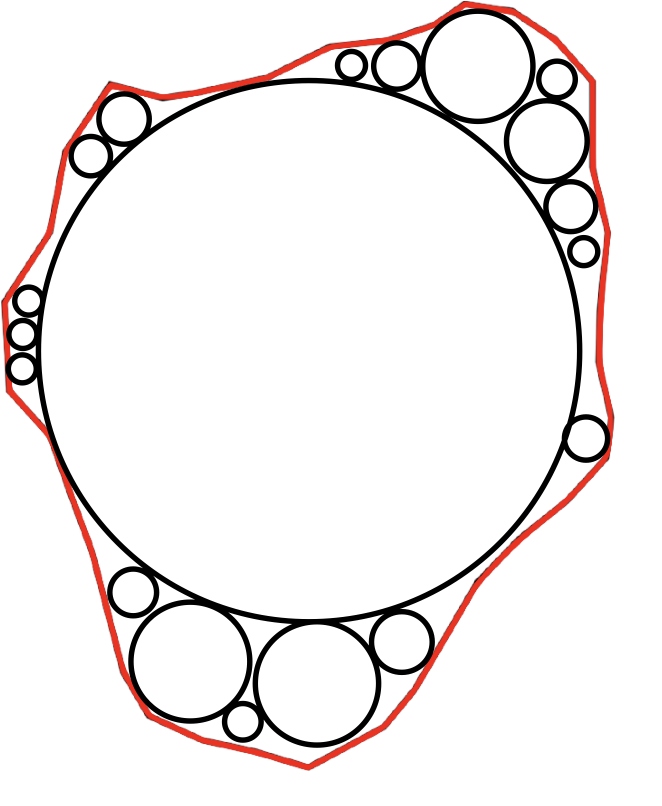
\includegraphics[width=5.8cm]{Images/clump1.png}
\subcaption{}
\label{fig:3figsA}}
\qquad
\begin{minipage}{7cm}
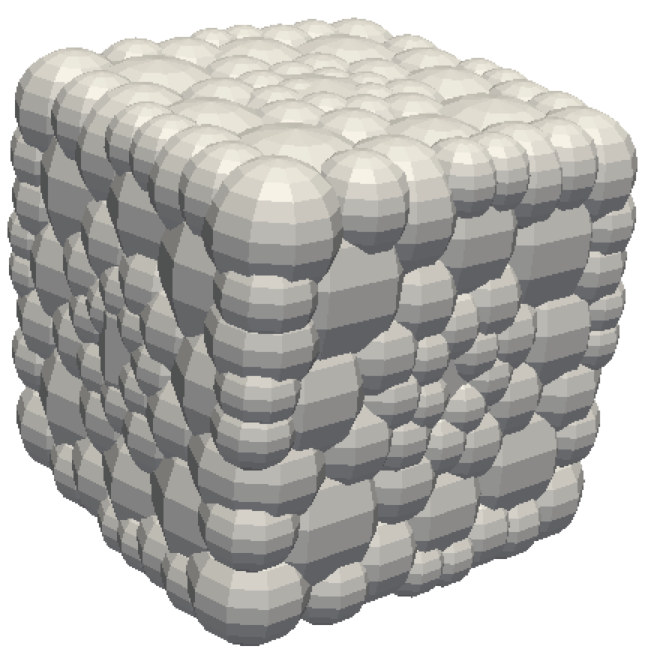
\includegraphics[width=7cm]{Images/clump2.png}
\subcaption{}
\label{fig:3figsB}
\end{minipage}
\caption{Clump example a) schematic representation of the solid, b) STL image of the solid body model}
\end{figure}
The particles motion formulated in Lagrangian frame of reference \cite{cundall1979discrete} with momentum and inertia equations:
\begin{equation}\label{solid_body_force}
m_{i} \frac{d \boldsymbol{u}_{\mathrm{p}, i}}{d t}= \mathbf{F}_{i,n} + \mathbf{F}_{i,t} + \mathbf{F}_{i,f} + \mathbf{F}_{i,b}
\end{equation}
\begin{equation}
I_{i} \frac{d \boldsymbol{\omega}_{\mathrm{p}, i}}{d t}= \mathbf{r}_{i,c}+\mathbf{F}_{i,t}+\mathbf{T}_{i,r},
\end{equation}
where $\mathbf{u}_{\mathrm{p}, i}$ - translational velocity of the particle $i$, $\boldsymbol{\omega}_{\mathrm{p}, i}$ - angular velocity of the particle $i$, $\mathbf{F}_{i,n}$ is the normal particle-particle contact force, $\mathbf{F}_{i,t}$ tangential particle-particle contact force. $\mathbf{F}_{i,f}$ force from surrounding fluid phase. All forces like gravity, electrostatic forces etc are summarised to $\mathbf{F}_{i,b}$ and $\mathbf{T}_{i,r}$ is an additional torque on the particle.

The second moment of inertia $I_p$ is essential for calculating stress, for the case of a sphere, it could be calculated as:
\begin{equation}
I_{p}=\frac{2 m_{p} r^{2}}{5}
\end{equation}
In this application, the discrete element method used from LIGGGHTS® package, which is an open-source software designed for simulating granular flows and their interactions. LIGGGHTS® is built on C++ and based on LAMMPS® molecular dynamics simulator.

\subsection{Time integration}

In LIGGGHTS \cite{kloss2011liggghts}, the second-order accurate Velocity-Verlet method is employed for time integration. The method consists of two steps. First, the particle position $r_i$ is integrated over the entire time step using the half-step velocity:
\begin{equation}
\mathbf{u}_{\mathbf{p},i}(t+\Delta t / 2)=\mathbf{u}_{\mathbf{p},i}(t)+\frac{\Delta t}{2} \frac{\partial \mathbf{u}_{\mathbf{p},i}}{\partial t}(t)
\end{equation}
\begin{equation}
\mathbf{r}(t+\Delta t)=\mathbf{r}(t)+\Delta t \mathbf{u}_{\mathbf{p},i}(t+\Delta t / 2)
\end{equation}
In the subsequent step, the remaining half-step of the velocity is integrated as follows:
\begin{equation}
\mathbf{u}_{\mathbf{p},i}(t+\Delta t)=\mathbf{u}_{\mathbf{p},i}(t+\Delta t / 2)+\frac{\Delta t}{2} \frac{\partial \mathbf{u}_{\mathbf{p},i}}{\partial t}(t+\Delta t / 2)
\end{equation}
Here, $\partial \mathbf{u}_{p,i}/dt(t+\Delta t)$ is evaluated from the acting forces as described in \ref{solid_body_force}. This two-step process ensures accurate time integration of particle positions and velocities, taking into account the forces acting on each particle.

\subsection{Particle–particle contact model}

The used method is based on the theory of Cundall and Strack\cite{cundall1979discrete}, where the complex collision behaviour of spheres is approximated by simple spring-dashpot interactions in normal ($n$) and tangential ($\tau$) direction as
\begin{equation}
\boldsymbol{F}_{i j}^{int}=\boldsymbol{F}_{i j}^{n} \cdot n_{i j}+\boldsymbol{F}_{i j}^{\tau} \cdot \tau_{i j}
\end{equation}
\begin{equation}
    \boldsymbol{F}_{\mathrm{n}}=k_{\mathrm{n}} \delta_{\mathrm{n}}-\eta_{\mathrm{n}} \boldsymbol{u}_{\mathrm{p}, \mathrm{n}}^{\mathrm{rel}}
\end{equation}
\begin{equation}
    \boldsymbol{F}_{\tau}=k_{\tau} \delta_{\tau}-\eta_{\tau} \boldsymbol{u}_{\mathrm{p},{\tau}}^{\mathrm{rel}}
\end{equation}
where $k$ is the spring coefficient from Hertz contact theory, $\delta_n$ the particle overlap, $\eta_{\tau}$ the viscous damping coefficient from Mindlin-Deresiewicz \cite{mindlin1953elastic} and $\mathbf{u}^{rel}$ the relative velocity of the colliding particles.

For a spherical particle, the moment of inertia \( I_i \) can be considered as a scalar because the sphere exhibits symmetry about all axes. In this case, the moment of inertia will be the same for any axis of rotation that passes through the sphere's center. This simplifies the mathematical description and calculations, as the direction of the axis of rotation doesn't need to be considered—the value of the moment of inertia will be constant in any case.

In vector form, the moment of inertia is usually represented by a tensor, which is generally a matrix. However, for a sphere, this matrix would be diagonal with identical diagonal elements, allowing it to be simplified to a scalar value.

\begin{figure}[!htp]
\centering
\parbox{7cm}{
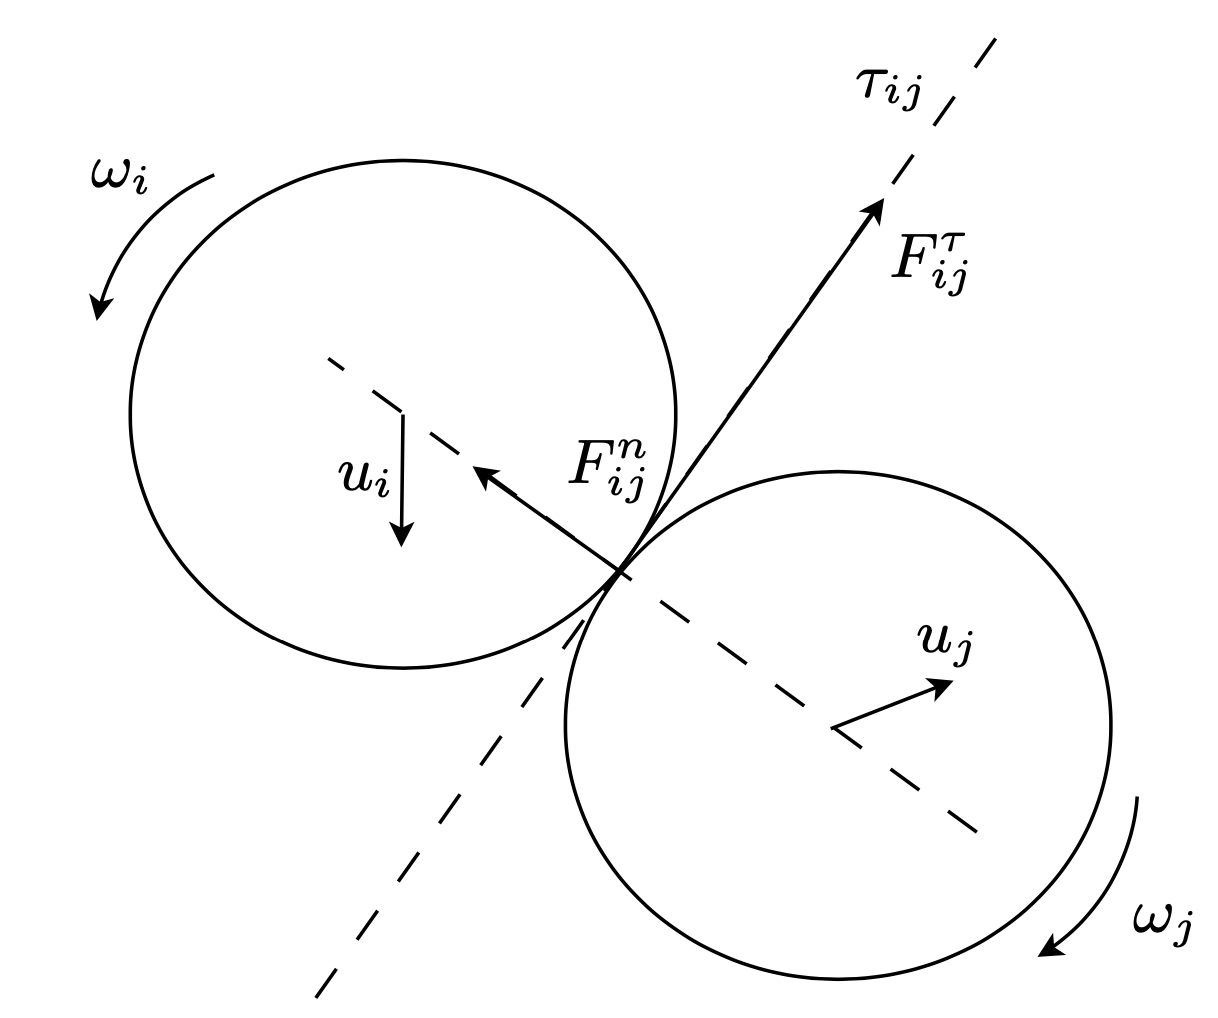
\includegraphics[width=7cm]{Images/particle_model_2.png}
\caption{Force directions for a multi-spherical body.}
\label{fig:2figsA}}
\qquad
\begin{minipage}{7cm}
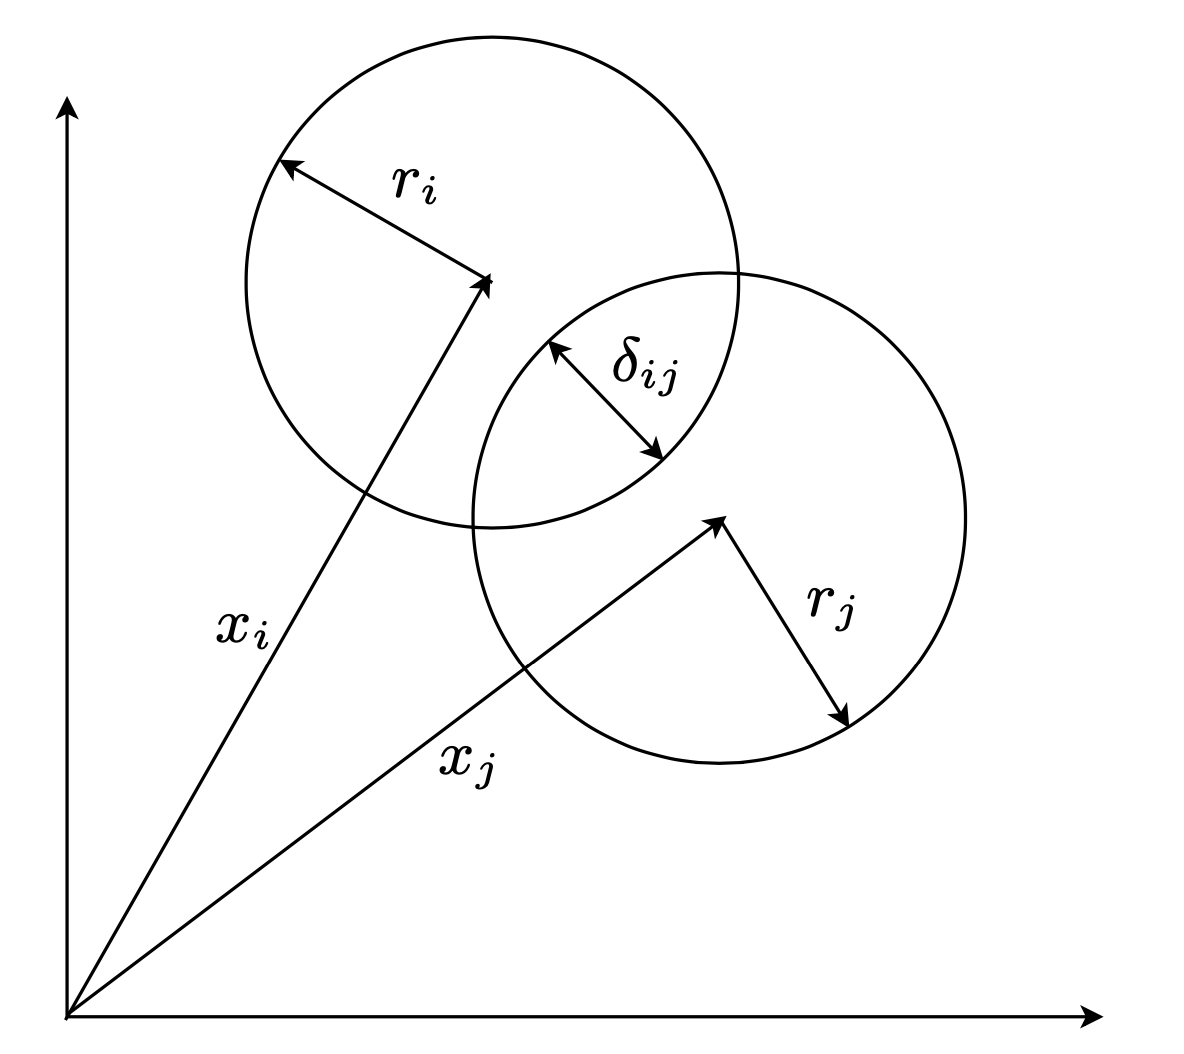
\includegraphics[width=7cm]{Images/particle_model.png}
\caption{Schematic representation of contact model for a multi-spherical body.}
\label{fig:2figsB}
\end{minipage}
\end{figure}
\begin{equation}
\begin{aligned}
k_{\mathrm{n}} & =\frac{4}{3} E_{\text {eff }} \sqrt{r_{\mathrm{eff}} \delta_{\mathrm{n}}} \\
k_{\tau} & =8 G_{\text {eff }} \sqrt{r_{\text {eff }} \delta_{n}}
\end{aligned}
\end{equation}
where $r_{\text {eff }}$ the effective radius, $E_{\text {eff }}$ Young’s modulus and $G_{\text {eff }}$ shear modulus, which defined for two colliding particles as:
\begin{equation}
\begin{aligned}
r_{\mathrm{eff}} & =\left(\frac{1}{r_i}+\frac{1}{r_j}\right)^{-1} \\
E_{\text {eff }} & =\left(\frac{1-\nu_{\mathrm{p}, i}^2}{E_i}+\frac{1-\nu_{\mathrm{p}, j}^2}{E_j}\right)^{-1} \\
G_{\text {eff }} & =\left(\frac{2-\nu_{\mathrm{p}, i}}{G_i}+\frac{2-\nu_{\mathrm{p}, j}}{G_j}\right)^{-1},
\end{aligned}
\end{equation}
where $\nu$ is the Poisson’s ratio and 
\begin{equation}
\begin{aligned}
 \eta_{\mathrm{n}} &= -\alpha(e) \sqrt{m_{\mathrm{eff}} k_{\mathrm{n}}} \\
 \eta_{\tau} &= -\alpha(e) \sqrt{\frac{2}{3}} m_{\mathrm{eff}} k_{\tau}
\end{aligned}
\end{equation}
more details could be found in \cite{LIGGGHTS} documentation.

\section{Coupling}
There are several methods which is available for solving the two-way coupling problem with CFDEMcoupling code, they listed below in increasing complexity order:
\begin{itemize}
\item The Immersed Boundary Method based on Distributed Lagrange Multipliers \cite{glowinski1999distributed} was introduced by Shirgaonkar \cite{shirgaonkar2009new}.
\item Hager \cite{hager2014cfd} adopted Shirgaonkar's approach, using solid body force correction with the PISO algorithm. The software implementation of this approach is provided as the CFDEMcoupling code \cite{kloss2012models}.
\item Blais \cite{blais2016semi} stores the solid body force as a separate field and adjusts the same implementation as Hager \cite{kloss2012models}.
\item The proposed approach in the current work for two-phase flow is based on the methods mentioned above and the VOF method with isoAdvector for free surface reconstruction.
\end{itemize}
In the paper by Balachandran et al. \cite{balachandran2021resolved}, a resolved CFD-DEM method was used for blood flow simulations. This work serves as an example of two-way coupling with a solid moving body having 6 degrees of freedom (DOF) for one fluid phase. The model of a red blood cell is treated as a cluster of overlapping spheres interconnected by a flexible mathematical bond. The inter-cellular interactions are modeled using a Hertz-Mendelian model, with attractive forces enforced through a cohesive force based on the Morse potential. A similar idea is used as the core concept for simulating granular media of artificial shape as rocks and boulders.

The resolved CFD-DEM method is technically an Immersed Boundary Method with a fictitious domain for the flow, where the DEM describes particle interactions. The full description of the system is as follows:

\begin{equation}
    \frac{\partial (\rho \mathbf{u})_i}{\partial t} + \nabla p_i  +  \nabla \cdot(\rho \mathbf{u}\mathbf{u})_i - \nabla \tau_i + \rho_i \mathbf{g} = \mathbf{f}_{s} \quad in ~\Omega_f \cup \Omega_a
\end{equation}
\begin{equation}
    \nabla\cdot \mathbf{u}_i = 0 \quad in ~\Omega_f \cup \Omega_a
\end{equation}
\begin{equation}
    \frac{\partial \alpha}{\partial t} + \nabla\cdot(\alpha\mathbf{u}_i) = 0 \quad in ~\Omega_f \cup \Omega_a
\end{equation}
\begin{equation}
    m_{p} \frac{\mathrm{d} \mathbf{u}_{\mathbf{p}}}{\mathrm{d} t}=m_{p} \mathbf{g}+F_{p}^{f}+\sum_{N_{p}} F_{p}^{p}+\sum_{N_{w}} F_{p}^{w}+F_{p}^{\mathrm{ext}} \\ \quad in ~\Omega_s
\end{equation}
\begin{equation}
    \mathbf{u} = \mathbf{u}_{\Gamma} \quad on \in \Gamma, \mathbf{u} = \mathbf{u}_p \quad on ~\Omega_s
\end{equation}
\begin{equation}
%\begin{array}{l}
I_{p} \frac{\mathrm{d} \omega_{\mathbf{p}}}{\mathrm{d} t}=\mathbf{r} \times\left(F_{p}^{f}+\sum_{N_{p}} F_{p}^{p}+\sum_{N_{w}} F_{p}^{w}+F_{p}^{\mathrm{ext}}\right)\\ \quad in ~\Omega_s
%\end{array}
\end{equation}
where  $\mathbf{f}_{s}$ - is a force from the solid body side which calculated with the DEM, $\Omega_f,\Omega_a$ -  is the volume taken by fluid and air correspondingly, $m_p$ - is the particle mass, $F^p_f$ is the hydrodynamic forces acting on the particle and $F^p_p$ and $F^w_p$ are the particle–particle and particle–wall interaction forces, respectively. $F^{ext}_p$ is the $p$ external force acting on the particle which comes from cohesion, adhesion and other interaction forces. $I_p$ is the second moment of inertia of the particle, ${\omega}_p$ is the angular velocity, and $r$ is the distance between the particle centroid and a point on the surface of the particle. 

There are two primary categories of CFD-DEM: unresolved and resolved. In the unresolved method, the particle size is significantly smaller than the computational cell. Here, the particles' motion is simulated as if they were another fluid, and this is solved using the Navier-Stokes momentum equation \cite{kloss2012models}. In contrast, in the resolved method, the particle size is considerably larger than the computational cell, as shown in the Figure \ref{fig:res_unres} below:
\begin{figure}[h]
    \centering
    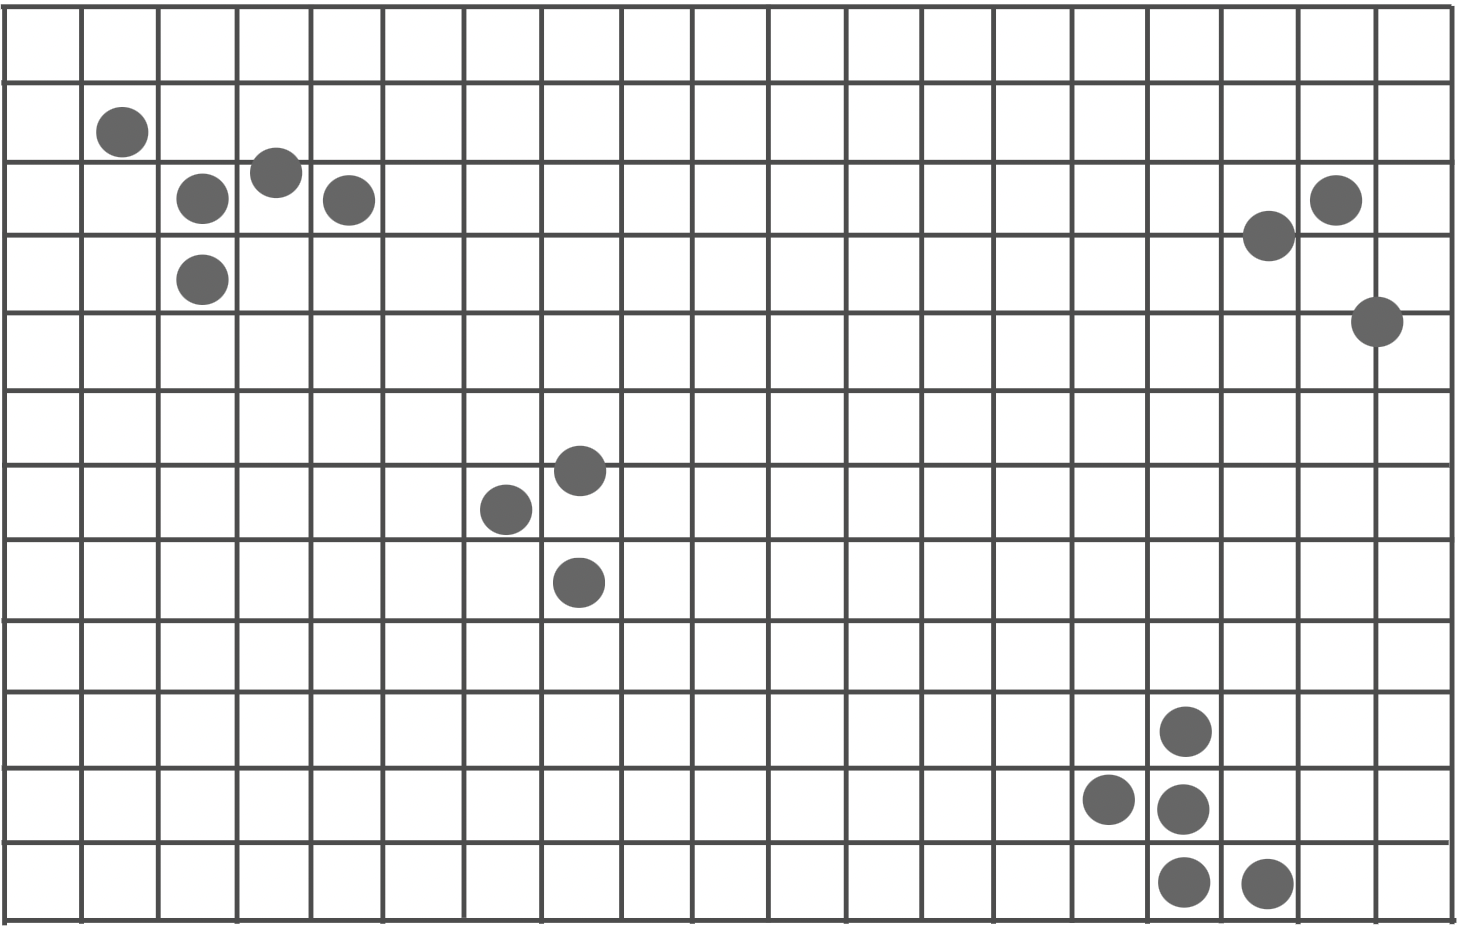
\includegraphics[width=11cm]{Images/resolved_cfddem.png}
    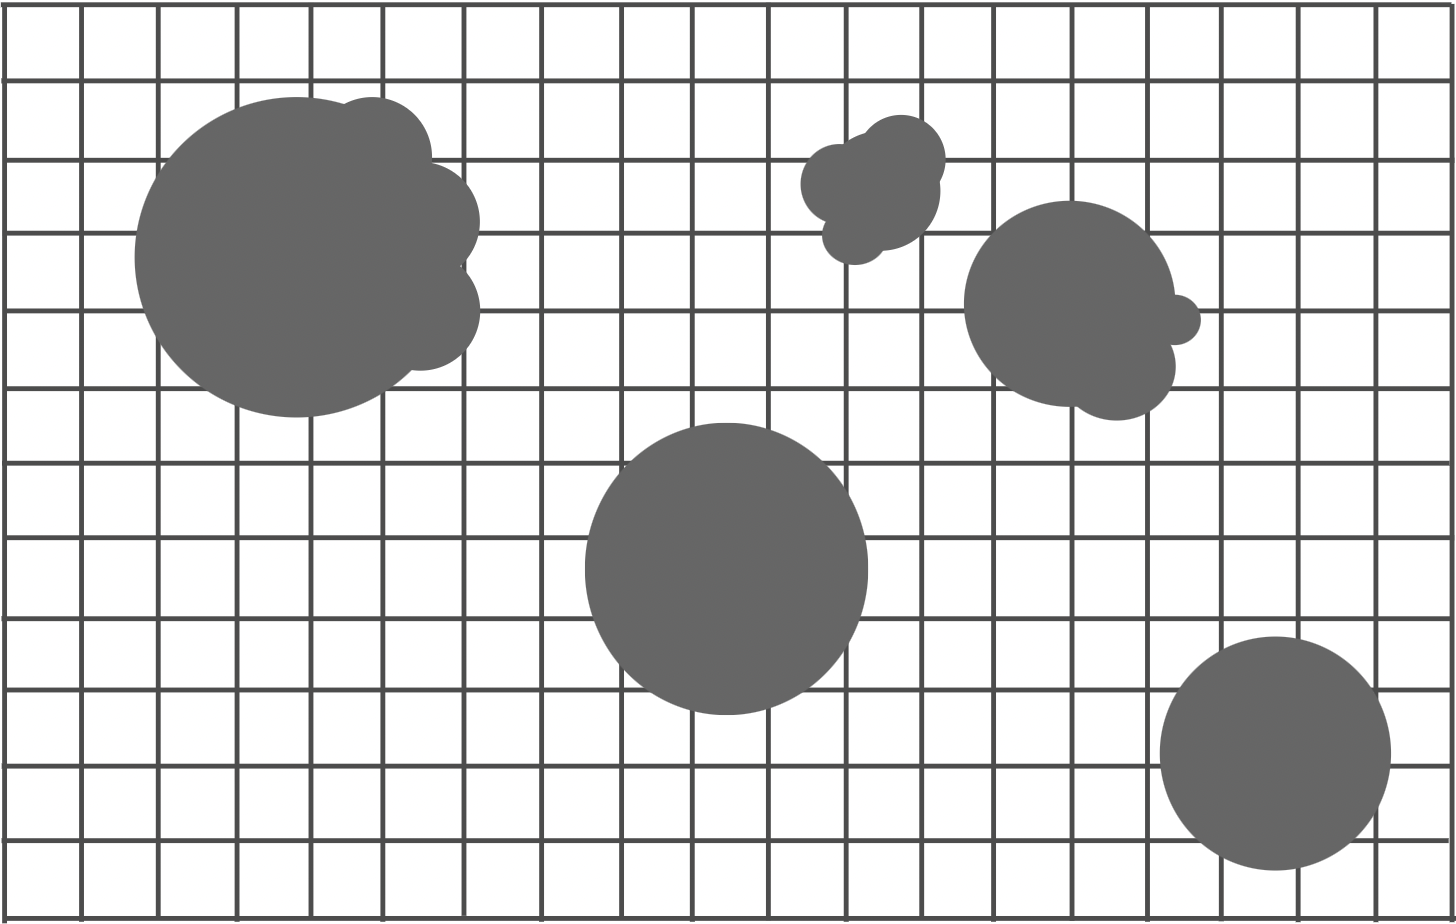
\includegraphics[width=11cm]{Images/unresolved_cfddem.png}
    \caption{Particle representation approaches}
    \label{fig:res_unres}
\end{figure}
For the resolved CFD-DEM there is two main approaches how to provide the coupling. One is direct forcing approach \cite{uhlmann2005immersed} which could be used to modify the flow with a no-slip boundary condition which change the particle velocity. The main feature of the approach is dependence on the spatial discretization which used for IB flux calculation because the velocity field have to be divergence free.

Another one is continuous forcing approach \cite{mittal2005immersed} where the source term from the solid body \ref{2.13} added before discretization, therefore no independence from spatial discretization.

\begin{equation}\label{2.13}
F_{B}=\frac{\rho \beta \left(\mathbf{u}_{\mathbf{p}}-\mathbf{u}_f\right)}{\kappa \Delta t}
\end{equation}
where $\mathbf{u}_f$ and $\mathbf{u}_p$ are fluid and particle velocity correspondingly. The solid volume fraction $\beta$ or so-called \textit{voidFraction}, $\beta = 1$ when the cell fully occupied with the solid, or $\beta = 0$ if it not occupied and at the interface $0 < \beta < 1$. %as schematically shown on the Fig
%ref{} privide a figure
$\kappa$ is the rigid body constraint.

Note that the method has been used for Fluid Structure Interaction (FSI) problems \cite{blais2016semi}, \cite{nan2023high}, \cite{mao2020resolved}, but original part is combination of two phase flow with surface reconstruction method interaction with solid bodies of arbitrary shape. 

\subsection{Force term calculation}

To account solid body forces \ref{IB_forces} during the computation of the system of governing equations we will add particle position data, save in \textit{voidFraction} field and with it as source term in momentum equation during calculation pressure and velocity cycle which is based on PISO algorithm, described before in \ref{p-v-coupling} section.

\textbf{step 1:} Prediction step, to find intermediate velocity will include body force calculated on previous time step:

\begin{equation}\label{NS_algebraic_1}
    a_{P}^{\mathrm{u}} \mathbf{u}_{P}+\sum_{N} a_{N}^{\mathrm{u}} \mathbf{u}_{N}= -\nabla p + \mathbf{F}^{m*}_i
\end{equation}
then let $\mathbf{H}(\mathbf{u})= -\sum_{N} a_{N}^{\mathrm{u}} \mathbf{u}_{N}$ and rewrite \ref{NS_algebraic_1} as
\begin{equation}\label{NS_algebraic_2}
    \begin{aligned}
a_{P}^{\mathrm{u}} \mathbf{u}_{P} &=\mathbf{H}(\mathbf{u})-\nabla p \\
\mathbf{u}_{P} &=\left(a_{P}^{\mathrm{u}}\right)^{-1}(\mathbf{H}(\mathbf{u})-\nabla p)
\end{aligned}
\end{equation}
where $P$ is an index arbitrary velocity node, $N$ is an index from neighbouring cells, $\mathbf{F}^{m*}_i$ - is immersed boundary forcing term. We also need to solve phase convection equation at this step.

\textbf{step 2:} Correction step,
Compute flux on a cell faces using Rhie-Chow \cite{rhie} correction
\begin{equation}
    \phi = \frac{H(\mathbf{u})}{a^u_P}\cdot S_f
\end{equation}
where $S_f$ is area of a cell face.
From \ref{NS_algebraic_1} to satisfy continuity equation $\nabla\cdot \mathbf{u} = 0$
\begin{equation}
    (a_{P}^{\mathbf{u}})^{-1} \cdot \nabla^2 p^* = \nabla \cdot \phi
\end{equation}
then correct the velocity field:
\begin{equation}
    \mathbf{u}^{*} = (a_{P}^{\mathbf{u}})^{-1}(H(\mathbf{u}) - \nabla p^* + \mathbf{F}^{m*}_i)
\end{equation}
where $\mathbf{u}^*$ and $p^*$,an intermediate velocity and a pressure. Finally, this forcing term is corrected using the difference between the current velocity and the prescribed one within the immersed body
\begin{equation}
\mathbf{F}_{i}^{m^{* *}} = \boldsymbol{F}_{i}^{m^{*}}+\frac{\alpha \beta_{i}}{\Delta t}\left(\boldsymbol{u}_{i b, i}-\boldsymbol{u}_{i}^{m^{* *}}\right)
\end{equation}
Then repeat step 2 until it converged or depends on how many correction steps we choose to run, after write down new velocity and pressure fields $\mathbf{u}^{m+1}$ and $p^{m+1}$ for the next step $m + 1$. Schematically algorithm shown on the Figure \ref{fig:diag_PISO} below.

\begin{figure}[!h]
    \centering
    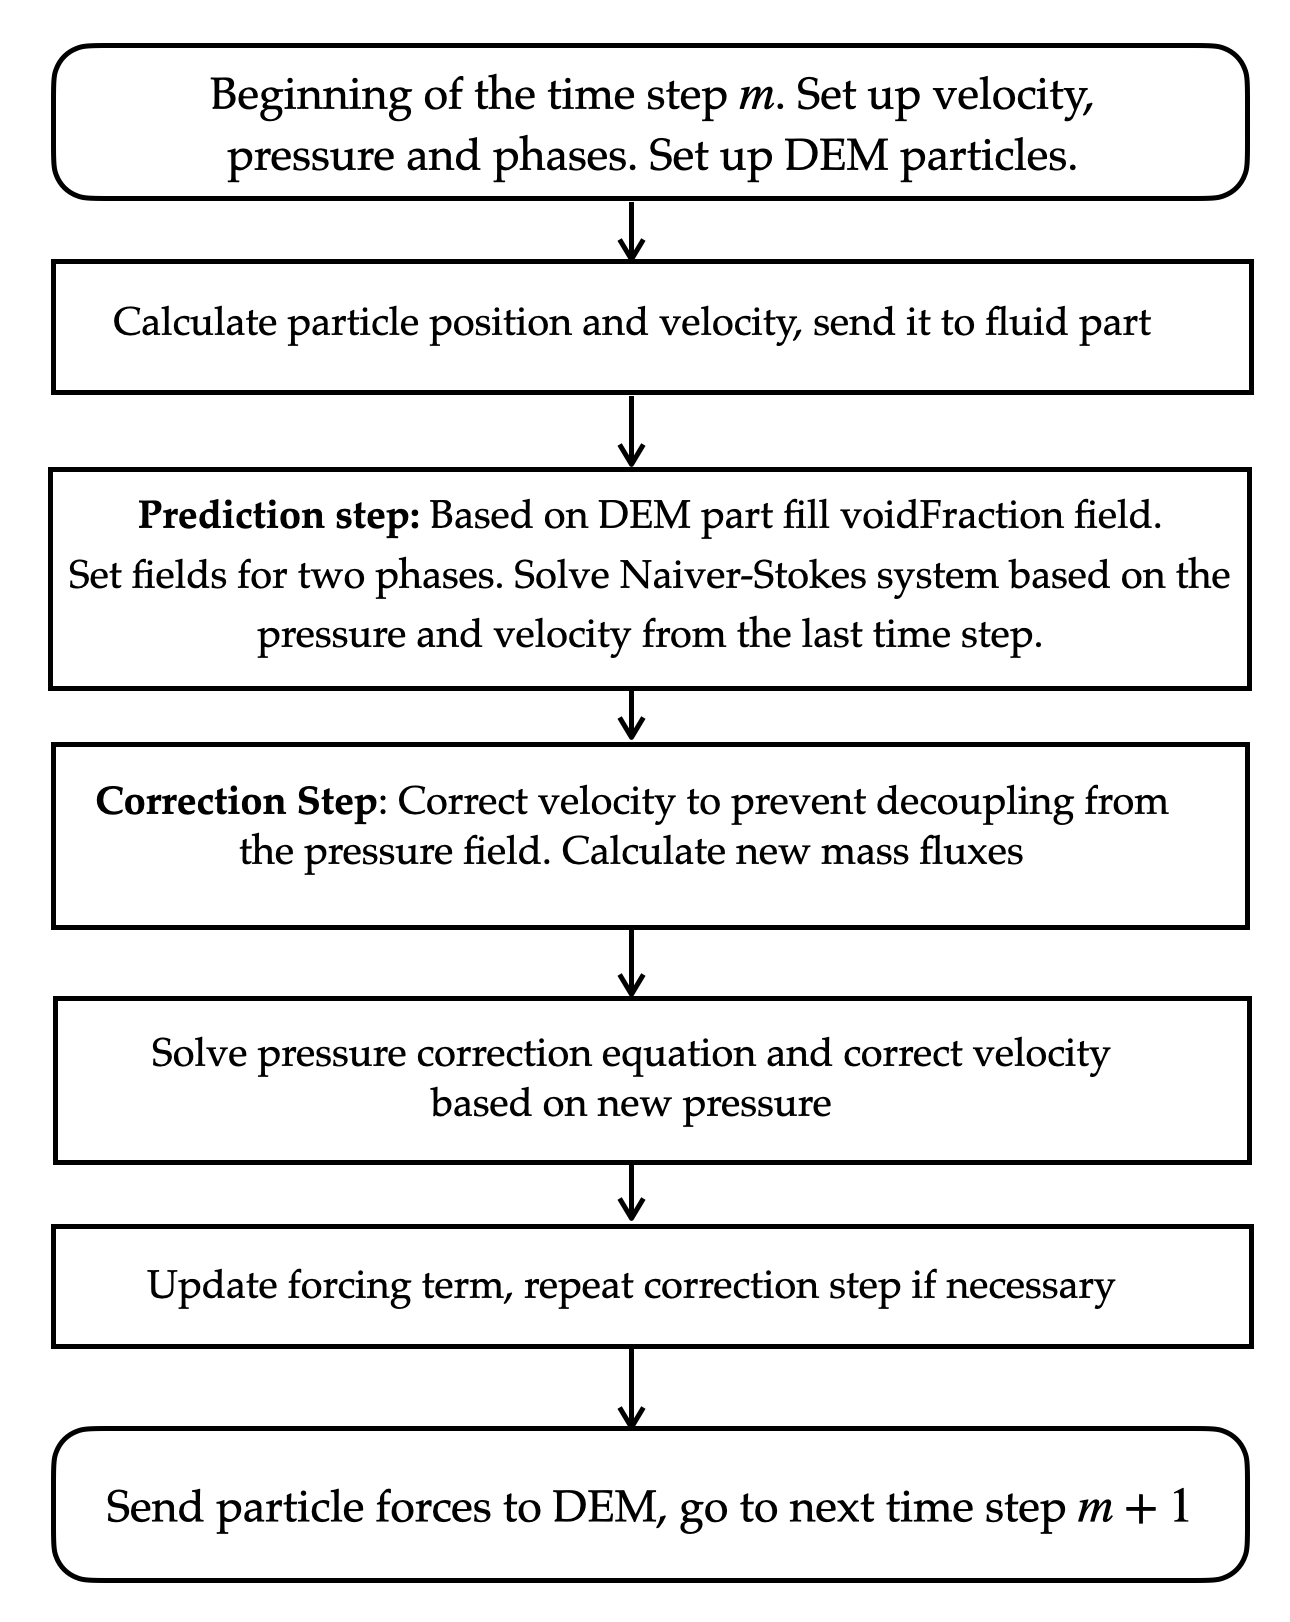
\includegraphics[width=12cm]{Images/chap3/diag_PISO.png}
    \caption{Schematic diagram for CFD-DEM algorithm.}
    \label{fig:diag_PISO}
\end{figure}

\section{Conclusion}
This chapter provided the final algorithm for coupling sold bodies and fluid parts. For the fluid part, we used the sharp interface VOF method - isoAdvector\cite{roenby2019isoadvector}. For simulation, the solid part Hertz particle-particle contact model is considered. We also provided examples of multispherical solid bodies proposed to be used in the algorithm as approximations of solid rocks for landslide simulation.
